
Let $\chi = \mathbb{R}$, and let $\pi(x)=cg(x)$, where $g(x)=e^{-|x|/10}(1+\cos(x)\sin(x))$, and let $h(x)=x+x^2$. With appropriate choise of $M,B, \sigma$, and starting distribution $\mathcal{L}(X_0)$, estimate $\mathbb{E}_\pi(h)$ in each of the two different ways:
(a) With a usual random-walk Metropolis algorithm for $\pi$, with the usual proposal distribution $Y_n$~$N(X_{n-1},\sigma^2)$.
For this problem, we choose again $M$ to be 10e+6 and $B$ to be 10e+5, and we choose $\sigma$ to be 53 so that the acceptance rate is around the optimal value 0.234.
The RWM algorithm is implemented using the following code:
\begin{knitrout}
\definecolor{shadecolor}{rgb}{0.969, 0.969, 0.969}\color{fgcolor}\begin{kframe}
\begin{alltt}
\hlcom{#Estimate E_pi(X+X^2) where pi=cg using RWM algorithm where}
\hlcom{# g(x) = e^(-|x|/10)*(1+cos(x)sin(x^3))}
\hlcom{# with increments following a N(0,sigma^2) distribution}

\hlstd{fn} \hlkwb{=} \hlkwa{function}\hlstd{(}\hlkwc{x}\hlstd{) \{x}\hlopt{+}\hlstd{x}\hlopt{^}\hlnum{2}\hlstd{\}}
\hlstd{g} \hlkwb{=} \hlkwa{function}\hlstd{(}\hlkwc{x}\hlstd{) \{}\hlkwd{exp}\hlstd{(}\hlopt{-}\hlkwd{abs}\hlstd{(x)}\hlopt{/}\hlnum{10}\hlstd{)}\hlopt{*}\hlstd{(}\hlnum{1}\hlopt{+}\hlkwd{cos}\hlstd{(x)}\hlopt{*}\hlkwd{sin}\hlstd{(x}\hlopt{^}\hlnum{3}\hlstd{))\}}

\hlstd{sigma} \hlkwb{=} \hlnum{53}
\hlstd{M} \hlkwb{=} \hlnum{1e+6}
\hlstd{B} \hlkwb{=} \hlnum{1e+5}

\hlcom{#initialization}
\hlstd{fnlist} \hlkwb{=} \hlkwd{numeric}\hlstd{(M}\hlopt{+}\hlstd{B)}
\hlstd{xlist} \hlkwb{=} \hlkwd{numeric}\hlstd{(M}\hlopt{+}\hlstd{B)}
\hlstd{x} \hlkwb{=} \hlkwd{rnorm}\hlstd{(}\hlnum{1}\hlstd{,}\hlnum{0}\hlstd{,sigma)}
\hlstd{acc} \hlkwb{=} \hlnum{0}

\hlkwa{for} \hlstd{(i} \hlkwa{in} \hlnum{1}\hlopt{:}\hlstd{(M}\hlopt{+}\hlstd{B)) \{}
  \hlstd{eps} \hlkwb{=} \hlkwd{rnorm}\hlstd{(}\hlnum{1}\hlstd{,}\hlnum{0}\hlstd{,sigma)}

  \hlkwa{if} \hlstd{(}\hlkwd{runif}\hlstd{(}\hlnum{1}\hlstd{)}\hlopt{<=}\hlkwd{g}\hlstd{(x}\hlopt{+}\hlstd{eps)}\hlopt{/}\hlkwd{g}\hlstd{(x)) \{}
    \hlkwa{if} \hlstd{(i}\hlopt{>}\hlstd{B)}
      \hlstd{acc}\hlkwb{=}\hlstd{acc}\hlopt{+}\hlnum{1}
    \hlstd{x} \hlkwb{=} \hlstd{x}\hlopt{+}\hlstd{eps}
  \hlstd{\}}
  \hlstd{xlist[i]} \hlkwb{=} \hlstd{x}
  \hlstd{fnlist[i]} \hlkwb{=} \hlkwd{fn}\hlstd{(x)}
\hlstd{\}}

\hlstd{funcmean} \hlkwb{=} \hlkwd{mean}\hlstd{(fnlist[(B}\hlopt{+}\hlnum{1}\hlstd{)}\hlopt{:}\hlstd{(M}\hlopt{+}\hlstd{B)])}
\hlstd{funciidse} \hlkwb{=} \hlkwd{sd}\hlstd{(fnlist[(B}\hlopt{+}\hlnum{1}\hlstd{)}\hlopt{:}\hlstd{(M}\hlopt{+}\hlstd{B)])}\hlopt{/}\hlkwd{sqrt}\hlstd{(M)}
\hlstd{acf_k} \hlkwb{=} \hlkwd{acf}\hlstd{(fnlist[(B}\hlopt{+}\hlnum{1}\hlstd{)}\hlopt{:}\hlstd{(M}\hlopt{+}\hlstd{B)],}\hlkwc{lag.max} \hlstd{=} \hlnum{1000}\hlstd{,}\hlkwc{plot} \hlstd{=} \hlnum{FALSE}\hlstd{)}\hlopt{$}\hlstd{acf}
\hlstd{varfact} \hlkwb{=} \hlnum{2}\hlopt{*}\hlkwd{sum}\hlstd{(acf_k[}\hlnum{1}\hlopt{:}\hlkwd{min}\hlstd{(}\hlkwd{which}\hlstd{(acf_k}\hlopt{<}\hlnum{0.05}\hlstd{))])}\hlopt{-}\hlnum{1}
\hlstd{funcse} \hlkwb{=} \hlstd{funciidse}\hlopt{*}\hlkwd{sqrt}\hlstd{(varfact)}
\hlstd{accrate} \hlkwb{=} \hlstd{acc}\hlopt{/}\hlstd{M}

\hlkwd{cat}\hlstd{(}\hlstr{'B = '}\hlstd{,B,}\hlstr{', M = '}\hlstd{,M,}\hlstr{'\textbackslash{}n'}\hlstd{)}
\hlkwd{cat}\hlstd{(}\hlstr{'Number of samples accepted = '}\hlstd{,acc,}\hlstr{', acceptance rate = '}\hlstd{,accrate,}\hlstr{'\textbackslash{}n'}\hlstd{)}
\hlkwd{cat}\hlstd{(}\hlstr{'Estimate = '}\hlstd{,funcmean,}\hlstr{'\textbackslash{}n'}\hlstd{)}
\hlkwd{cat}\hlstd{(}\hlstr{'i.i.d. standard error = '}\hlstd{,funciidse,}\hlstr{'\textbackslash{}n'}\hlstd{)}
\hlkwd{cat}\hlstd{(}\hlstr{'varfact = '}\hlstd{,varfact,}\hlstr{'\textbackslash{}n'}\hlstd{)}
\hlkwd{cat}\hlstd{(}\hlstr{'Standard error = '}\hlstd{,funcse,}\hlstr{'\textbackslash{}n'}\hlstd{)}
\end{alltt}
\end{kframe}
\end{knitrout}
Output of several runs:
\begin{knitrout}
\definecolor{shadecolor}{rgb}{0.969, 0.969, 0.969}\color{fgcolor}\begin{kframe}
\begin{verbatim}
## B =  1e+05 , M =  1e+06 
## Number of samples accepted =  238066 , acceptance rate =  0.238066 
## Estimate =  200.6944 
## i.i.d. standard error =  0.4448528 
## varfact =  6.844363 
## Standard error =  1.163812
## B =  1e+05 , M =  1e+06 
## Number of samples accepted =  237394 , acceptance rate =  0.237394 
## Estimate =  199.571 
## i.i.d. standard error =  0.4484531 
## varfact =  6.913195 
## Standard error =  1.179116
## B =  1e+05 , M =  1e+06 
## Number of samples accepted =  238054 , acceptance rate =  0.238054 
## Estimate =  200.1975 
## i.i.d. standard error =  0.4433383 
## varfact =  6.77882 
## Standard error =  1.154283
## B =  1e+05 , M =  1e+06 
## Number of samples accepted =  238477 , acceptance rate =  0.238477 
## Estimate =  200.3298 
## i.i.d. standard error =  0.4522812 
## varfact =  7.017603 
## Standard error =  1.198127
## B =  1e+05 , M =  1e+06 
## Number of samples accepted =  237175 , acceptance rate =  0.237175 
## Estimate =  198.6471 
## i.i.d. standard error =  0.4413461 
## varfact =  6.776058 
## Standard error =  1.148862
\end{verbatim}
\end{kframe}
\end{knitrout}
The tabulated result is as follows:\\
\begin{center}
\begin{knitrout}
\definecolor{shadecolor}{rgb}{0.969, 0.969, 0.969}\color{fgcolor}
\begin{tabular}{r|r|r|r|r}
\hline
estimation & acc\_rate & seiid & varfact & standard\_error\\
\hline
200.6944 & 0.238066 & 0.4448528 & 6.776058 & 1.163812\\
\hline
199.5710 & 0.237394 & 0.4484531 & 6.776058 & 1.179116\\
\hline
200.1975 & 0.238054 & 0.4433383 & 6.776058 & 1.154283\\
\hline
200.3298 & 0.238477 & 0.4522812 & 6.776058 & 1.198127\\
\hline
198.6471 & 0.237175 & 0.4413461 & 6.776058 & 1.148862\\
\hline
\end{tabular}


\end{knitrout}
\end{center}
We notice that the varfact values are quite small, indicating that the samples are not strongly correlated. To verify the effectiveness of the sampler, here we plot the value of $x$ after the burn-in stage
\begin{figure}[H]
  \centering
\begin{knitrout}
\definecolor{shadecolor}{rgb}{0.969, 0.969, 0.969}\color{fgcolor}\begin{kframe}
\begin{alltt}
\hlstd{xlist8a} \hlkwb{=} \hlstd{xlist}
\hlkwd{plot}\hlstd{(xlist8a[(B}\hlopt{+}\hlnum{1}\hlstd{)}\hlopt{:}\hlstd{(B}\hlopt{+}\hlstd{M)],}\hlkwc{type}\hlstd{=}\hlstr{'l'}\hlstd{)}
\end{alltt}
\end{kframe}
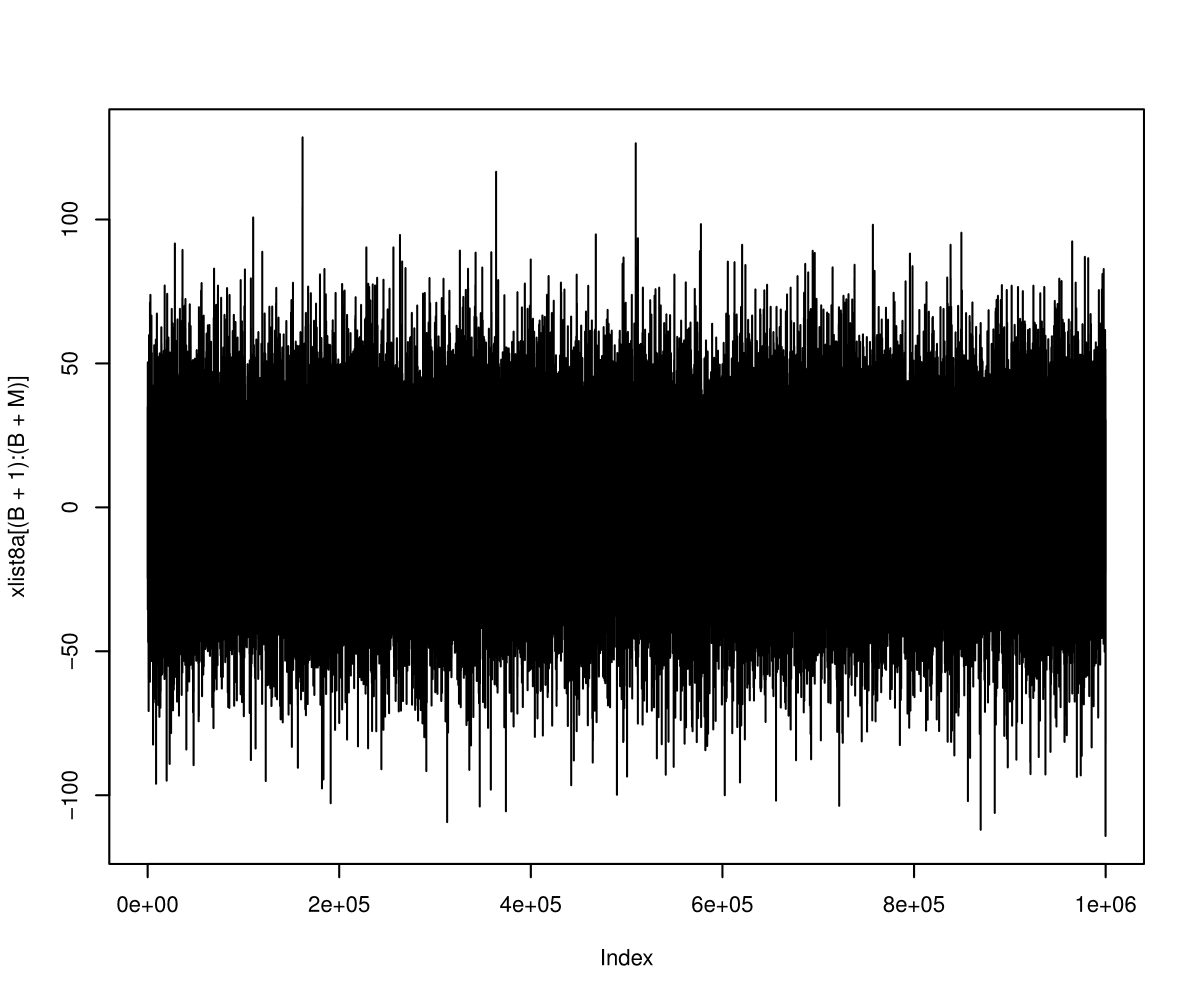
\includegraphics[width=\maxwidth]{figure/p8aplot-1} 

\end{knitrout}
		\caption{$x$ values of RWM algorithm after burning-in}
\end{figure}
From the figure above, we can see that the sample is reasonably well represented because of the high variability and low correlation, indicating a good (accurate) approximation by the RWM algorithm.\\
